\chapter{Numerical Results in the Time-Driven Approach}
This chapter is dedicated to presenting the results obtained by applying the Stochastic Reachability approach (discussed in Chapter \ref{chpt:Model_Description}) to the asset allocation problem. We recall that the output of the ODAA algorithm (see Theorem (\ref{thm:rec_algo})) is a sequence of allocation maps $\pi^{\star}=\{\mu_0^{\star},\ldots,\mu_{N-1}^{\star}\}$. For any portfolio realization $x \in \mathbb{R}$ at time $k \in \mathbb{N}$, the maps $\mu_k^{\star}$ provides us with the optimal asset allocation $\mu_k^{\star}(x)=\bm{u}_k^{\star}$; for instance, if $\bm{u}_k^{\star}= \begin{bmatrix}
0.2 & 0.2 & 0.6
\end{bmatrix}^T$, this means that 20\% of investor's wealth should be allocated to the first asset class, 20\% to the second one and the remaining 60\% to the third one. Objective of this chapter is to see what form these maps have at different time instant. The chapter unfolds as follows: in Section \ref{sec:The_Dataset} the dataset is presented and summarized by some sample statistics, in Section \ref{sec:Allocation_Maps} the parameters of the asset allocation problems are set and the allocation maps for the different models discussed in Chapter \ref{chpt:assetclass_returns} are reported. Moreover, the ODAA strategy will be compared with other famous asset allocation strategies such as the Constant-Mix and the \gls{CPPI}.

\section{The Dataset}\label{sec:The_Dataset}
Our asset class menu consists of cash, bond and equity. To represent these markets we adopt the indexes presented in Table \ref{tab:indexes}.
\begin{table}[]
	\centering
	\begin{tabular}{@{}lll@{}} \toprule
		Label & Asset Class & Index\\ \midrule
		C & Money Market & iShares Short Treasury Bond ETF\\
		\addlinespace[0.5em]
		B & US Bond  & Northern US Treasury Index \\
		\addlinespace[0.5em]
	    E &	US Equity &  {S\&P 500}\\ \bottomrule
		\addlinespace[0.5em]
	\end{tabular}
	\caption{Asset class and relative index}
	\label{tab:indexes}
\end{table}
The dataset is composed of weekly time series from 23 January 2010 to 15 April 2016. The data is downloaded from Yahoo Finance which is also where the reader is referred for more details of index composition. Asset class statistical indicators are summarized in Figure \ref{fig:assetclassReturns} and Table \ref{tab:sampleStatistics}. By comparing the annualized Mean return, it is clear that asset class Equity leads to higher performance than Bond and Bond, in turn, ensures higher performance than Cash. The annualized volatility tells us that the same hierarchy holds true also in terms of riskiness, being Equity the riskiest investment and Cash the least risky. Higher sample moments (Skewness and Kurtosis) suggest that the multivariate return distribution diverges significantly from a Gaussian one. Indeed, a quantitaive proof of this fact is given us from the Henze-Zirkler multivariate normality test which exhibits a zero p-value. 
\begin{figure}[h]\label{fig:assetclassReturns}
	\centering
	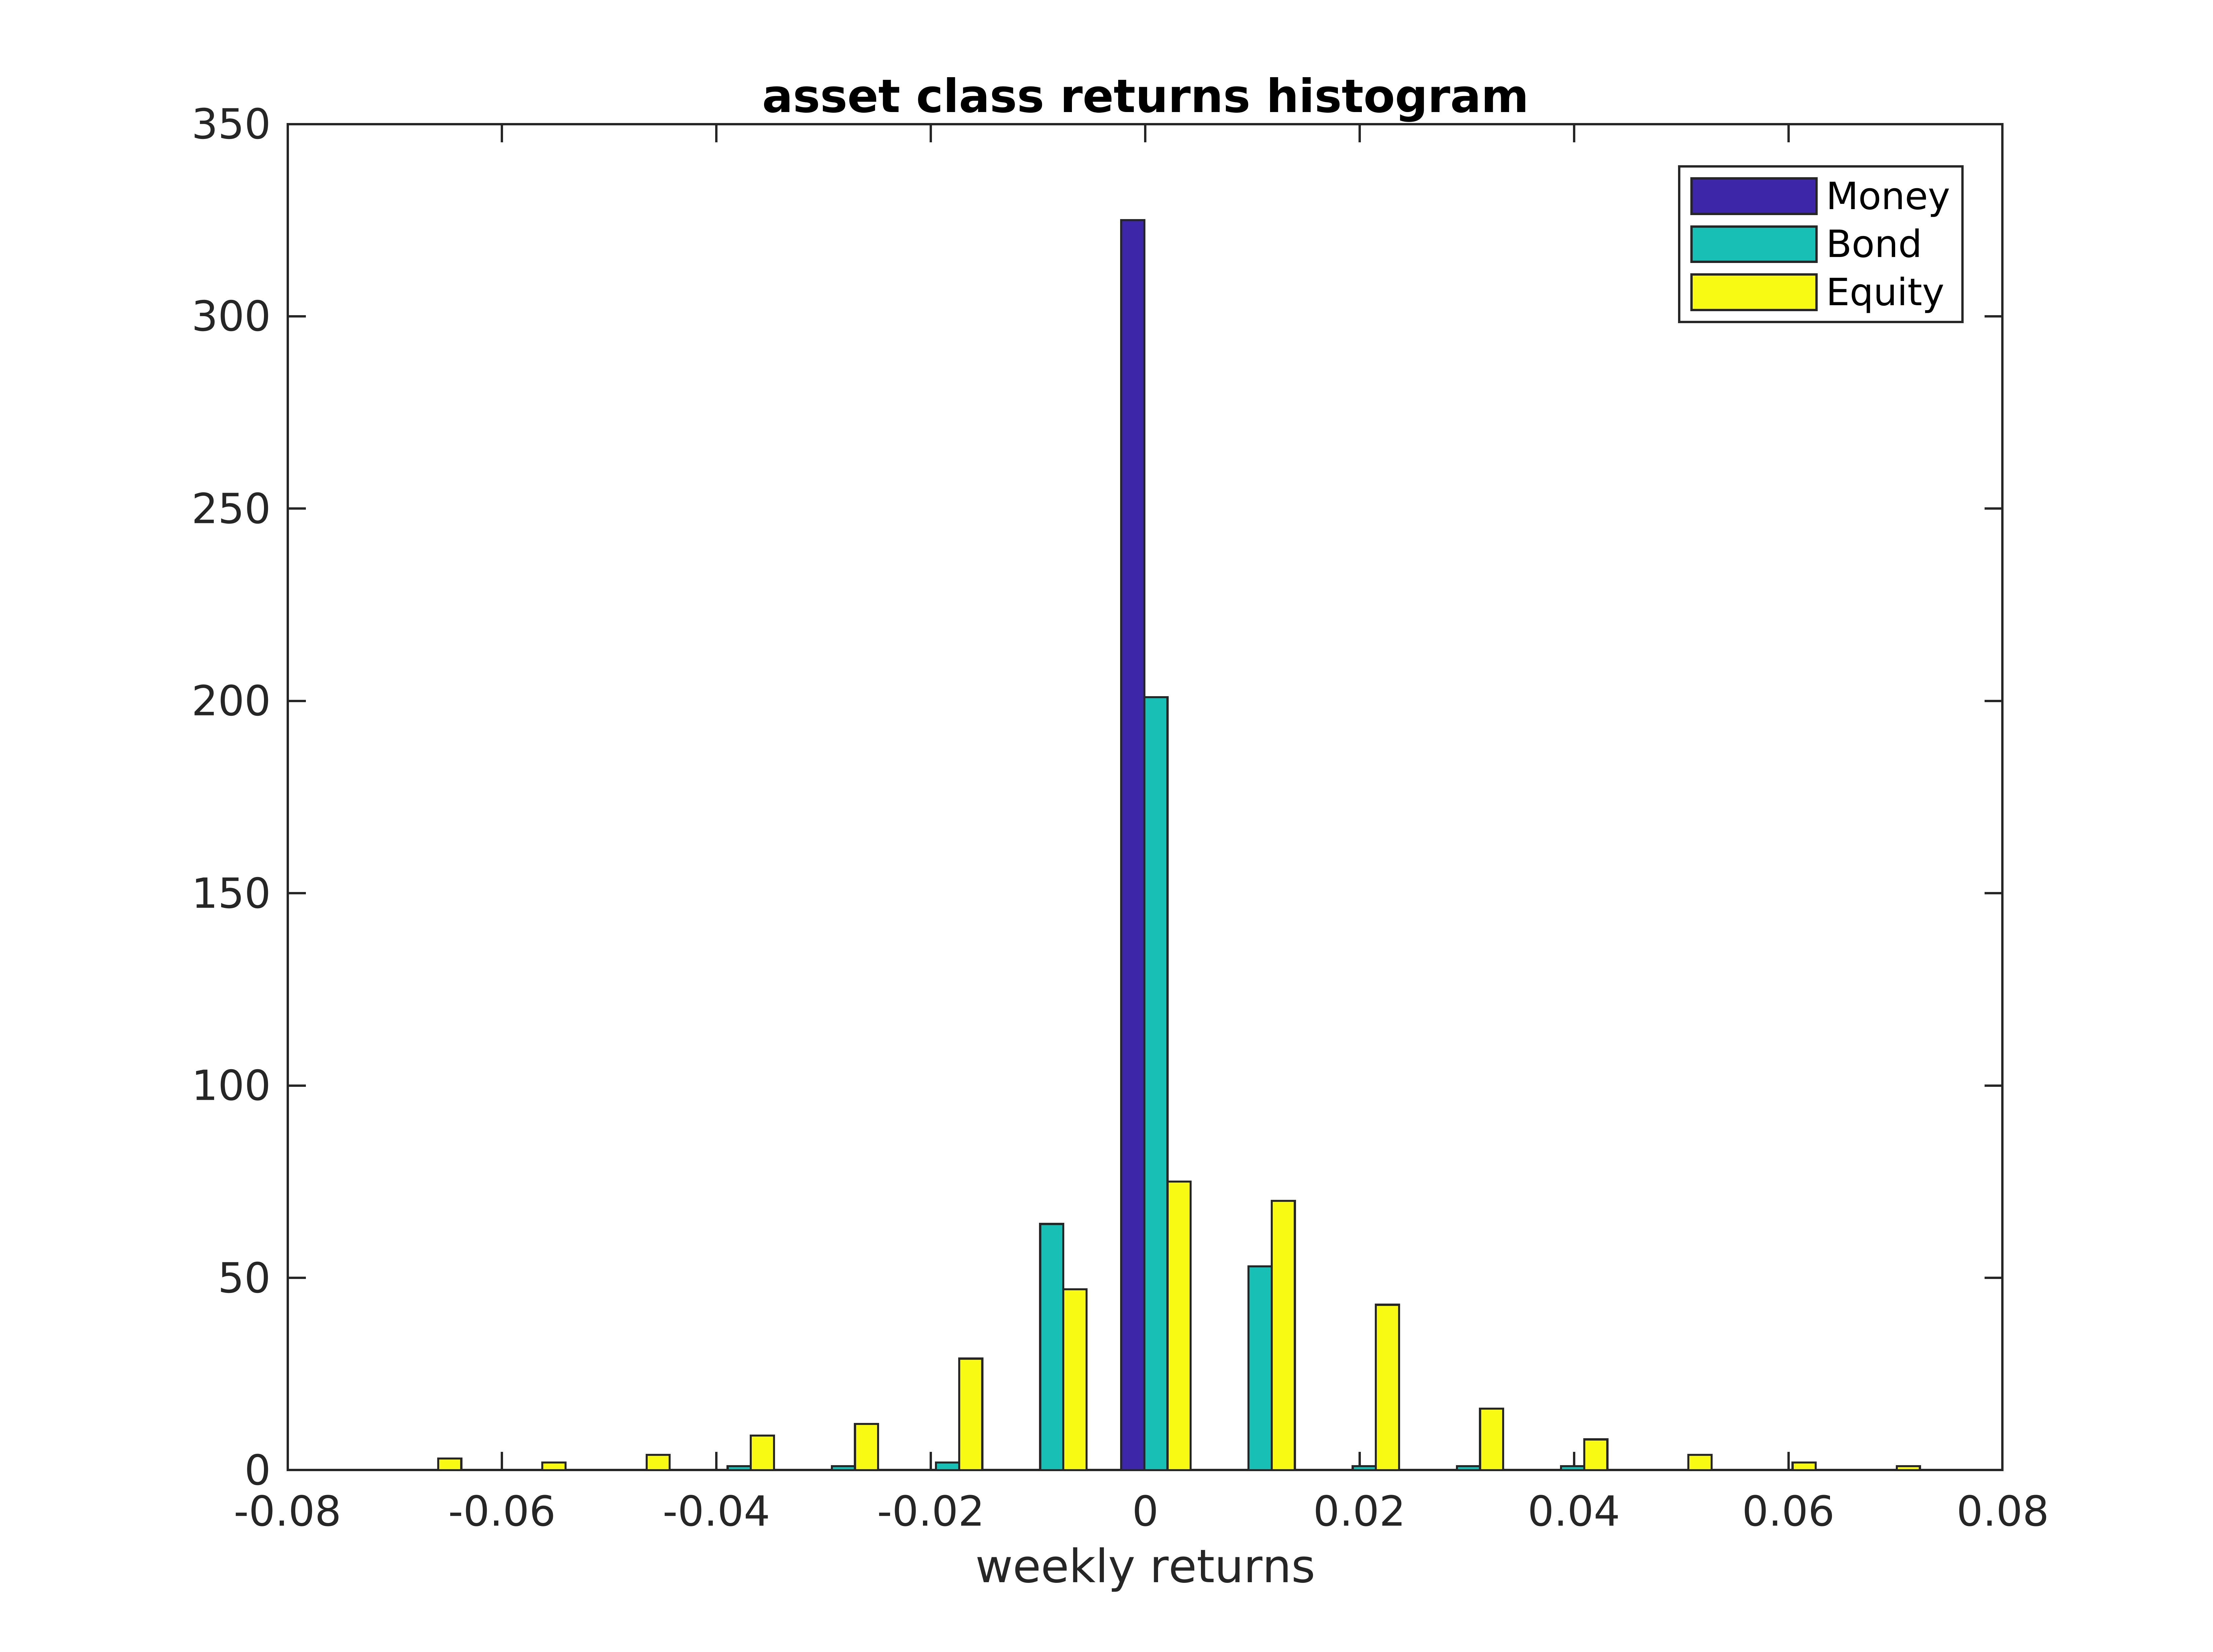
\includegraphics[scale=0.6]{Images/ReturnsHist.png}
	\caption{Weekly asset class returns histogram.}
\end{figure}
\begin{table}[h]
	\centering
	\begin{tabular}{@{}llll@{}} \toprule
		Statistic & C & B & E \\ \midrule
		Mean Return (ann) & 0.064\%  & 3.46\% & 12.11\%\\
		\addlinespace[0.5em]
		Volatility (ann) & 0.113\%  & 4.81\% & 14.81\% \\
		\addlinespace[0.5em]
		Median (ann) &	0\% & 4.58\% & 17.74\% \\
		\addlinespace[0.5em]
		Skewnwss & 0.262 & -0.0621 & -0.36 \\
		\addlinespace[0.5em]
		Kurtosis & 3.90 & 10.62 & 4.42 \\
		\addlinespace[0.5em]
		Monthly $V@R_{0.95}$ & 0.0808\% & 3.73\% & 14.95\%\\
		\addlinespace[0.5em]
		Max Drawdown & 0.106\% & 5.87\% & 23.98\% \\
		\addlinespace[0.5em]
		Mean Drawdown & 0.020\% & 1.5\% & 4.62\% \\
		\addlinespace[0.5em]
		Sharpe ratio & 0 & 0.692 & 0.767 \\ \bottomrule
		\addlinespace[0.5em]
	\end{tabular}
	\caption{Asset class returns sample statistics}
	\label{tab:sampleStatistics}
\end{table}

Finally, the sample correlation matrix is  
\[ 
\begin{bmatrix}
1 & 0.166 & -0.075 \\
  &  1    & -0.454 \\
  &       &  1
\end{bmatrix}.
\]

\section{Optimal Allocation Maps}\label{sec:Allocation_Maps}
Let us consider an asset allocation problem characterized by the following parameters:
\begin{itemize}
	\item 2-year investment horizon
	\item weekly rebalancing frequency, which means $N=104$ portfolio rebalancings
	\item monthly value-at-risk equals to 7\%
	\item target return $\theta=7\%$ per year
	\item initial wealth $x_0 = 1$
\end{itemize}
The target sets we want our portfolio value to stay within are 
\begin{align*}
X_0 & = \{1\}\\
X_k & = [0,\infty) \quad k = 1,\ldots,103 \\
X_{104} & = [(1+\theta)^2,\infty) = [1.07^2,\infty)
\end{align*}
In practice, these sets are discretized with a discretization step of $10^{-3}$ and truncated where the probability measure is negligible; the actual sets used in the implementation thus are $X_k = [0.5,1.9]$ $k=1,\ldots,103$, $X_{104}=[(1.07)^2,1.9]$. As stated in Problem \ref{prb:ODAA}, we are looking for a sequence of allocation maps which maximize the following joint probability
\[ \mathbb{P}\big(\{\omega \in \Omega : x_0 \in X_0,\ldots,x_{104} \in X_N \} \big).\]
The final choice to be made before running the algorithm is picking a model for the asset class returns. As a first example, we opt for the GM model which has been fitted to data applying the Expectation-Maximization method (see Subsection \ref{subsec:EM}). The parameter estimates are:

\begin{align}
\label{eq:GMparam1}
\bm{\mu}_1 & = 
\begin{bmatrix}
\num{1.054e-5} \\
\num{3.713e-4} \\
\num{2.298e-3}
\end{bmatrix}
\quad & \bm{\Sigma}_1 &= 
\begin{bmatrix}
\num{2.437e-8} & \num{1.266e-7} & \num{-2.365e-7} \\
& \num{3.596e-5}  & \num{-5.944e-5} \\
&                & \num{4.232e-4}
\end{bmatrix} \\
\bm{\mu}_2 & = \begin{bmatrix}
\num{2.115e-4} \\
\num{3.105e-2} \\
\num{-8.266e-3}
\end{bmatrix}
\quad & \bm{\Sigma}_2 &= 
\begin{bmatrix}
\num{2.372e-8} & \num{-7.961e-7} & \num{1.277e-6} \\
& \num{2.9e-5}  & \num{-4.411e-5} \\
&                & \num{6.949e-5}
\end{bmatrix}
\label{eq:GMparam2}
\end{align}
and $\lambda = 0.9908$.
By applying the backward algorithm enunciated in Theorem \ref{thm:rec_algo} we obtained 103 allocation maps, some of which are reported in Figure \ref{fig:mapsMixture}.
\begin{figure}[]
	\makebox[\textwidth][c]{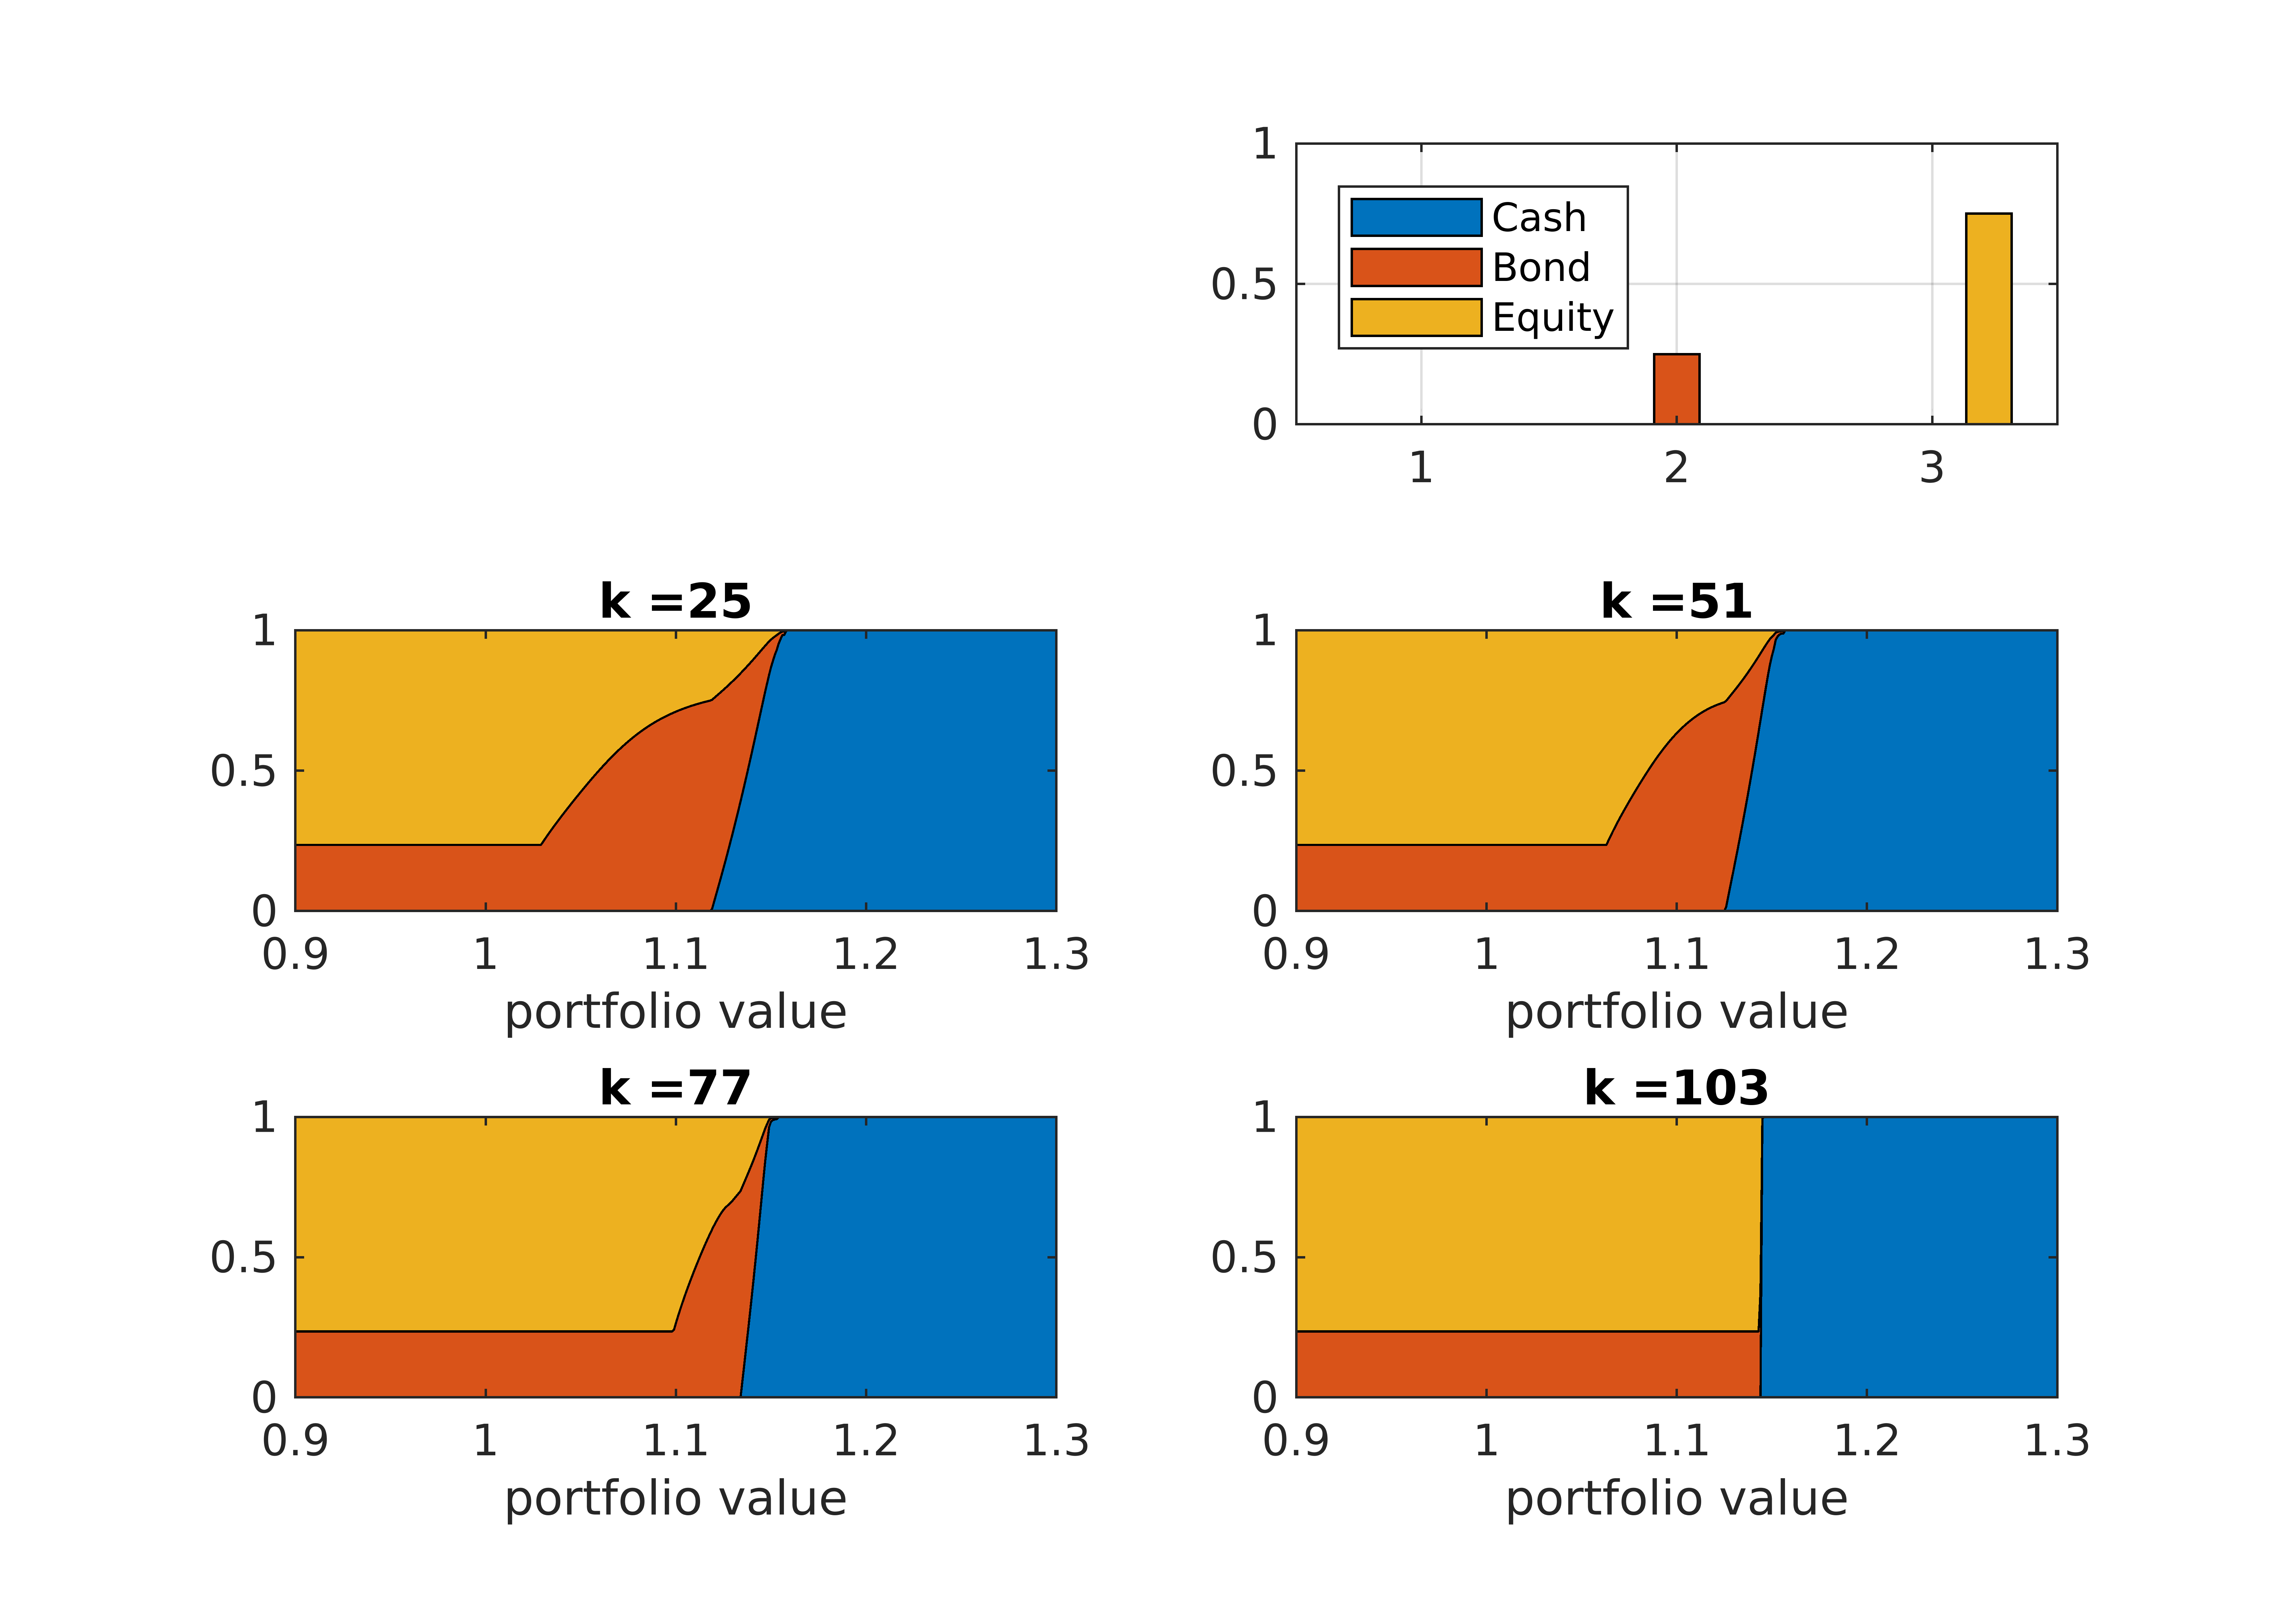
\includegraphics[scale =1]{Images/mapsMixturewk.png}}
	\caption{Optimal allocation maps, weekly rebalancing, GM model}
	\label{fig:mapsMixture}
\end{figure}


Let us now take the time to analyze the kind of investment strategy these maps imply. At the beginning of the investment ($k=0$), the optimal strategy prescribes that 25\% of investor's wealth be invested in Bond and 75\% in Equity. After 25 weeks, depending on the realization of portfolio value (x-axis in Figure \ref{fig:mapsMixture}), the optimal strategy tells us to allocate wealth as follows: if the portfolio is underperforming (e.g. its value is approximately below 1.029), the optimal allocation is a mix of Equity and Bond, that is the riskiest mix allowed (a 100\% allocation in Equity is not permitted due to the \text{risk} constraint). As soon as performance gets better (i.e. from \$1.029 to \$1.16) the Equity weight decreases in favor of more Bond and from a certain point on also Cash. When the portfolio is outperforming (i.e. above \$ 1.16), the whole wealth is invested in Cash, namely the least risky of the three asset classes. This kind of investing strategy is known in the literature with the name of \textit{contrarian} strategy. The name stems from the fact that contrarian investors bet against the prevailing market trend, namely they try to sell "high" and buy "low". Contrarian strategies perform well in volatile markets and poorly in trending market due to their \textbf{concave} nature (see \cite{Perold1988}). The optimal strategy obtained by the ODAA algorithm exhibits the same pattern also at successive rebalancing times, the only difference is that it becomes more extreme while approaching the investment end; for instance, at time $k=103$ there is no transition from the riskiest allocation to the least risky one. This behavior could be synthesized by saying that if the target has not been reached before the last week, the strategy will do whatever it takes to get there by assuming the riskiest exposure.

 The joint probability of reaching investor's goal is $J(x_0) = p^{\star} = 78.72\%$. This result is verified by running a Monte-Carlo simulation with $10^5$ draws at each rebalancing period from a GM distribution with parameters \ref{eq:GMparam1} and \ref{eq:GMparam2}, the joint probability obtained is $p_{MC} = 78.73\%$. Another interesting feature of the ODAA strategy is that $p^{\star}$ increases as the rebalancing frequency decreases. By looking at Table \ref{tab:ODAA_results}, it can be seen that as we move from a quarterly rebalancing frequancy\footnote{the problem of switching from a rebalancing frequency to another has been tackled as follows: the model is calibrated to weekly data, then linear returns are approximated by log-returns enabling us to write additive relations such as $w_{monthly} = w_{wk1}+\ldots+w_{wk4}$. Finally, using the hypothesis if iid returns we analytically derive the distribution of monthly and quarterly returns for the G, GM and NIG model. All this models are closed under convolution. } to a monthly one the optimal probability goes from 69.52\% to 73.35\%, and the same happens from monthly to weekly. This fact is rather intuitive since the more rebalancings the more chances to steer the portfolio within the target sets. It should be noted however, that in practice transaction costs have not a negligible impact on portfolio profitability when rebalancing is frequent. This is the reason why investment policies that update portfolio weights only when an "event" occurs are particularly appealing (they will be treated in Part \ref{part:2}).
 
 
\begin{table}[]
	%\renewcommand{\arraystretch}{0.5}
	\centering
	\resizebox{\textwidth}{!}{\begin{tabular}{@{}*{10}{c}@{}}
		\toprule
		& \multicolumn{3}{c}{G} & \multicolumn{3}{c}{GM} & \multicolumn{3}{c}{NIG} \\
		\addlinespace[0.5em]
		\cmidrule(l){2-4} \cmidrule(l){5-7} \cmidrule(l){8-10} 
		& wk & m & q 	& wk & m & q 	& wk & m & q\\
		\addlinespace[0.5em]
	$p^{\star}$ & 79.67\% & 75.56\% & 73.26\% & 78.59\%  & 73.20\% & 69.44\% & 78.53\% & 73.24\% &69.47\%  \\
	\addlinespace[0.5em]
	$p_{MC}$ & 79.77\% & 75.56\% & 73.28\% & 78.82\%  & 73.21\% & 69.58\% & 78.76\% & 73.30\% &69.32\%  \\
	\addlinespace[0.5em]	
	time[h] & 0.712 & 0.157 & 0.050 & 0.857  & 0.316 & 0.283 & 6.131 & 1.467 &0.371  \\	\bottomrule
	\end{tabular}}
	\caption{Probability of reaching the target set obtained via  ODAA algorithm ($p^{\star}$) and Monte-Carlo simulation ($p_{MC}$) for the Gaussian (GM), Gaussian Mixture (GM) and Normal Inverse Gaussian (NIG) model. Time is the computational time of the ODAA algorithm in hours.}
	\label{tab:ODAA_results}
\end{table}

\begin{table}[]
	\centering
	\begin{tabular}{@{}*{4}{c}@{}}
		\toprule
		& G & GM & NIG \\
		%\addlinespace[0.5em]
		\midrule	
		$\log L^{\star}$ & 4396.2& 4455.0  & 4481.4\\
		\addlinespace[0.5em]	
		\bottomrule
	\end{tabular}
	\caption{Log-likelihood for G, GM and NIG model}
	\label{tab:LogL_models}
\end{table}

Next, we used also the Gaussian and the NIG model to describe the asset class returns distribution. From Table (\ref{tab:LogL_models}) we see that the best fitting is provided by the GM model since it exhibits the highest Log-likelihood function value, nonetheless the NIG comes right after it. It is not surprising that the Gaussian model is ranked last as we were well-aware that the data considered deviates from a multivariate Gaussian sample (see Table \ref{tab:sampleStatistics}).
%\begin{wraptable}{l}{6cm}
%	\centering
%	\begin{tabular}{@{}*{5}{c}@{}}
%		\toprule
%	Moment	& G & GM & NIG & Empirical\\
%		\addlinespace[0.5em]
%		\midrule	
%	$\mu_{x_{k+1}}$	& & & \\
%	\addlinespace[0.5em]	
%	$\sigma_{x_{k+1}}$	& & & \\
%	\addlinespace[0.5em]
%	$\gamma_{x_{k+1}}$	& & & \\
%	\addlinespace[0.5em]
%	$\kappa_{x_{k+1}}$	& & & \\
%	\addlinespace[0.5em]
%	\bottomrule
%	\end{tabular}
%\end{wraptable}


\subsection{ODAA vs CPPI vs Constant-Mix}
Within the class of asset allocation strategies, the \gls{CPPI} and the Constant-Mix are among the most popular ones (see \cite{Perold1988}). After briefly discussing how they work, we will compare their performance to the ODAA's one.
\paragraph{CPPI}
The idea behind the \gls{CPPI} is to maintain the portfolio \textbf{exposure} to the risky asset, $E_k$, a constant multiple $m$ of the portfolio \textbf{cushion}, $C_k$. The risky asset is assume to be a mix of Bond and Equity. The cushion at time $k$ is defined as
\[
C_k = \max\big\{x_k-F_k,0 \big\}
\]
where $x_k$ is the portfolio value at time $k$ and $F_k$ is the so-called portfolio \textbf{floor}. The floor is a value below which the investor does not want the portfolio value to fall. In our case, the floor is a risk-free asset which grows deterministically at the Cash rate. Therefore, once the investor has specified 
\begin{itemize}
	\item an initial allocation $\bm{u}_0$ 
	\item the initial floor $F_0$ 
	\item a cushion multiplier $m$
	\item the maximum value-at-risk ($V@R_{1-\alpha}$) according to his risk profile,
\end{itemize}
he can synthesized the \gls{CPPI} strategy as follows
\begin{equation*}
\begin{aligned}
& \underset{\bm{u}_k}{\text{maximize}} & &  A\bm{u}_k \\
& \text{subject to} & & \bm{u}_k^T\bm{1}=1, \\
& & & u_i \geq 0 \qquad \forall i \in \{1,2,3\},\\
& & &\bm{u}_k\bm{\Lambda}\bm{u}_k \leq \sigma_{max}^2,\\
& & & \underbrace{xA\bm{u}_k}_{E_k} \leq mC_k.
\end{aligned}
\end{equation*}
where $A=\begin{bmatrix}0 & 1 & 1\end{bmatrix}$, $\sigma_{max}=\frac{V@R_{1-\alpha}}{z_{1-\alpha}}$, $x \in X_k$ and $k = 1,\ldots,N$. From this formulation we see that the investor aims at maximizing the allocation in the risky asset (matrix $A$ selects the allocation in Bond and Equity) while keeping under control the riskiness of the overall allocation and limiting the risky exposure to $m$ times the cushion. The covariance matrix $\bm{\Lambda}$ depends on the model chosen to describe the asset class returns distribution. In our analysis, we set $m=6$, $\bm{u}_0$ equal to the initial ODAA allocation, $F_0$ is chosen in such a way that also the initial exposure is $m$ times the cushion and the asset class return random vector follows a GM distribution with parameters (\ref{eq:GMparam1}) and (\ref{eq:GMparam2}). The others investment parameters are equal to the ones in the ODAA case. The CPPI allocation maps are reported in Figure \ref{fig:mapsMixtureCPPI}.



\paragraph{Constant-Mix}
Following a Constant-Mix strategy means maintaining an exposure to the risky asset that is a constant proportion of wealth. For instance, suppose one decides to keep a 60/40 proportion between risky ans risk-free asset. After a rebalancing time, asset prices change causing the portfolio proportion to change as well. Let us suppose that the risky asset has increased its price while the risk-free has fall. At the next rebalancing time, the Constant-Mix policy prescribes to sell shares of the risky asset and buy shares of the risk-free in order to recover the 60/40 mix. The constant mix is chosen by solving the following equivalent formulation of the Markowitz problem
\begin{equation*}
\begin{aligned}
& \underset{\bm{u}}{\text{maximize}} & &  \bm{u}^T\bm{\mu} \\
& \text{subject to} & & \bm{u}^T\bm{1}=1, \\
& & & u_i \geq 0 \qquad \forall i \in \{1,2,3\},\\
& & &\bm{u}\bm{\Lambda}\bm{u} \leq \sigma_{max}^2.\\
\end{aligned}
\end{equation*}
where $\sigma_{max}=\frac{V@R_{1-\alpha}}{z_{1-\alpha}}$ and $\bm{\mu}$ and $\bm{\Lambda}$ are the mean and the covariance matrix of the random vector $\bm{w}_{k+1}$ which represents the asset class returns.
The distribution of $\bm{w}_{k+1}$ could be any of the ones discussed in Chapter \ref{chpt:assetclass_returns}. The optimization problem has been solves assuming a GM distribution with parameters (\ref{eq:GMparam1}) and (\ref{eq:GMparam2}); the optimal constant mix is
\[ \bm{u}^{\star} = \begin{bmatrix} 0 & 0.2352 & 0.7648 \end{bmatrix}^T.\]


The ODAA and Constant-Mix belongs to the \textbf{concave} allocations strategies (see \cite{Plasse2013}). This means that their policy is to buy risky assets (Equity and Bond) when they fall and sell them when they raise. Concave strategies perform well in oscillating markets. Conversely, the \gls{CPPI} is an example of a \textbf{convex} strategy: risky assets are bought when they raise and sold when they fall. This behavior is clear from the allocation maps in Figure \ref{fig:mapsMixtureCPPI}. When portfolio performance is up, a more risky position is taken, when it is down, risky assets are sold and a more covered position is taken. Convex strategies perform well in trending markets.

In order to compare the performance of this three different strategies we ran a Monte-Carlo simulation. Starting from an initial wealth $x_0=1$, $\num{2e5}$ portfolio trajectories are drawn assuming a GM distribution with parameters (\ref{eq:GMparam1}) and (\ref{eq:GMparam2}) for vectors $\bm{w}_{k+1}$. Performance and risk figures are reported in table \ref{tab:MC_statistics}. The empirical density function of the 2-year investment return is reported in Figure \ref{fig:epirical_densities}.








\begin{figure}[]
	\makebox[\textwidth][c]{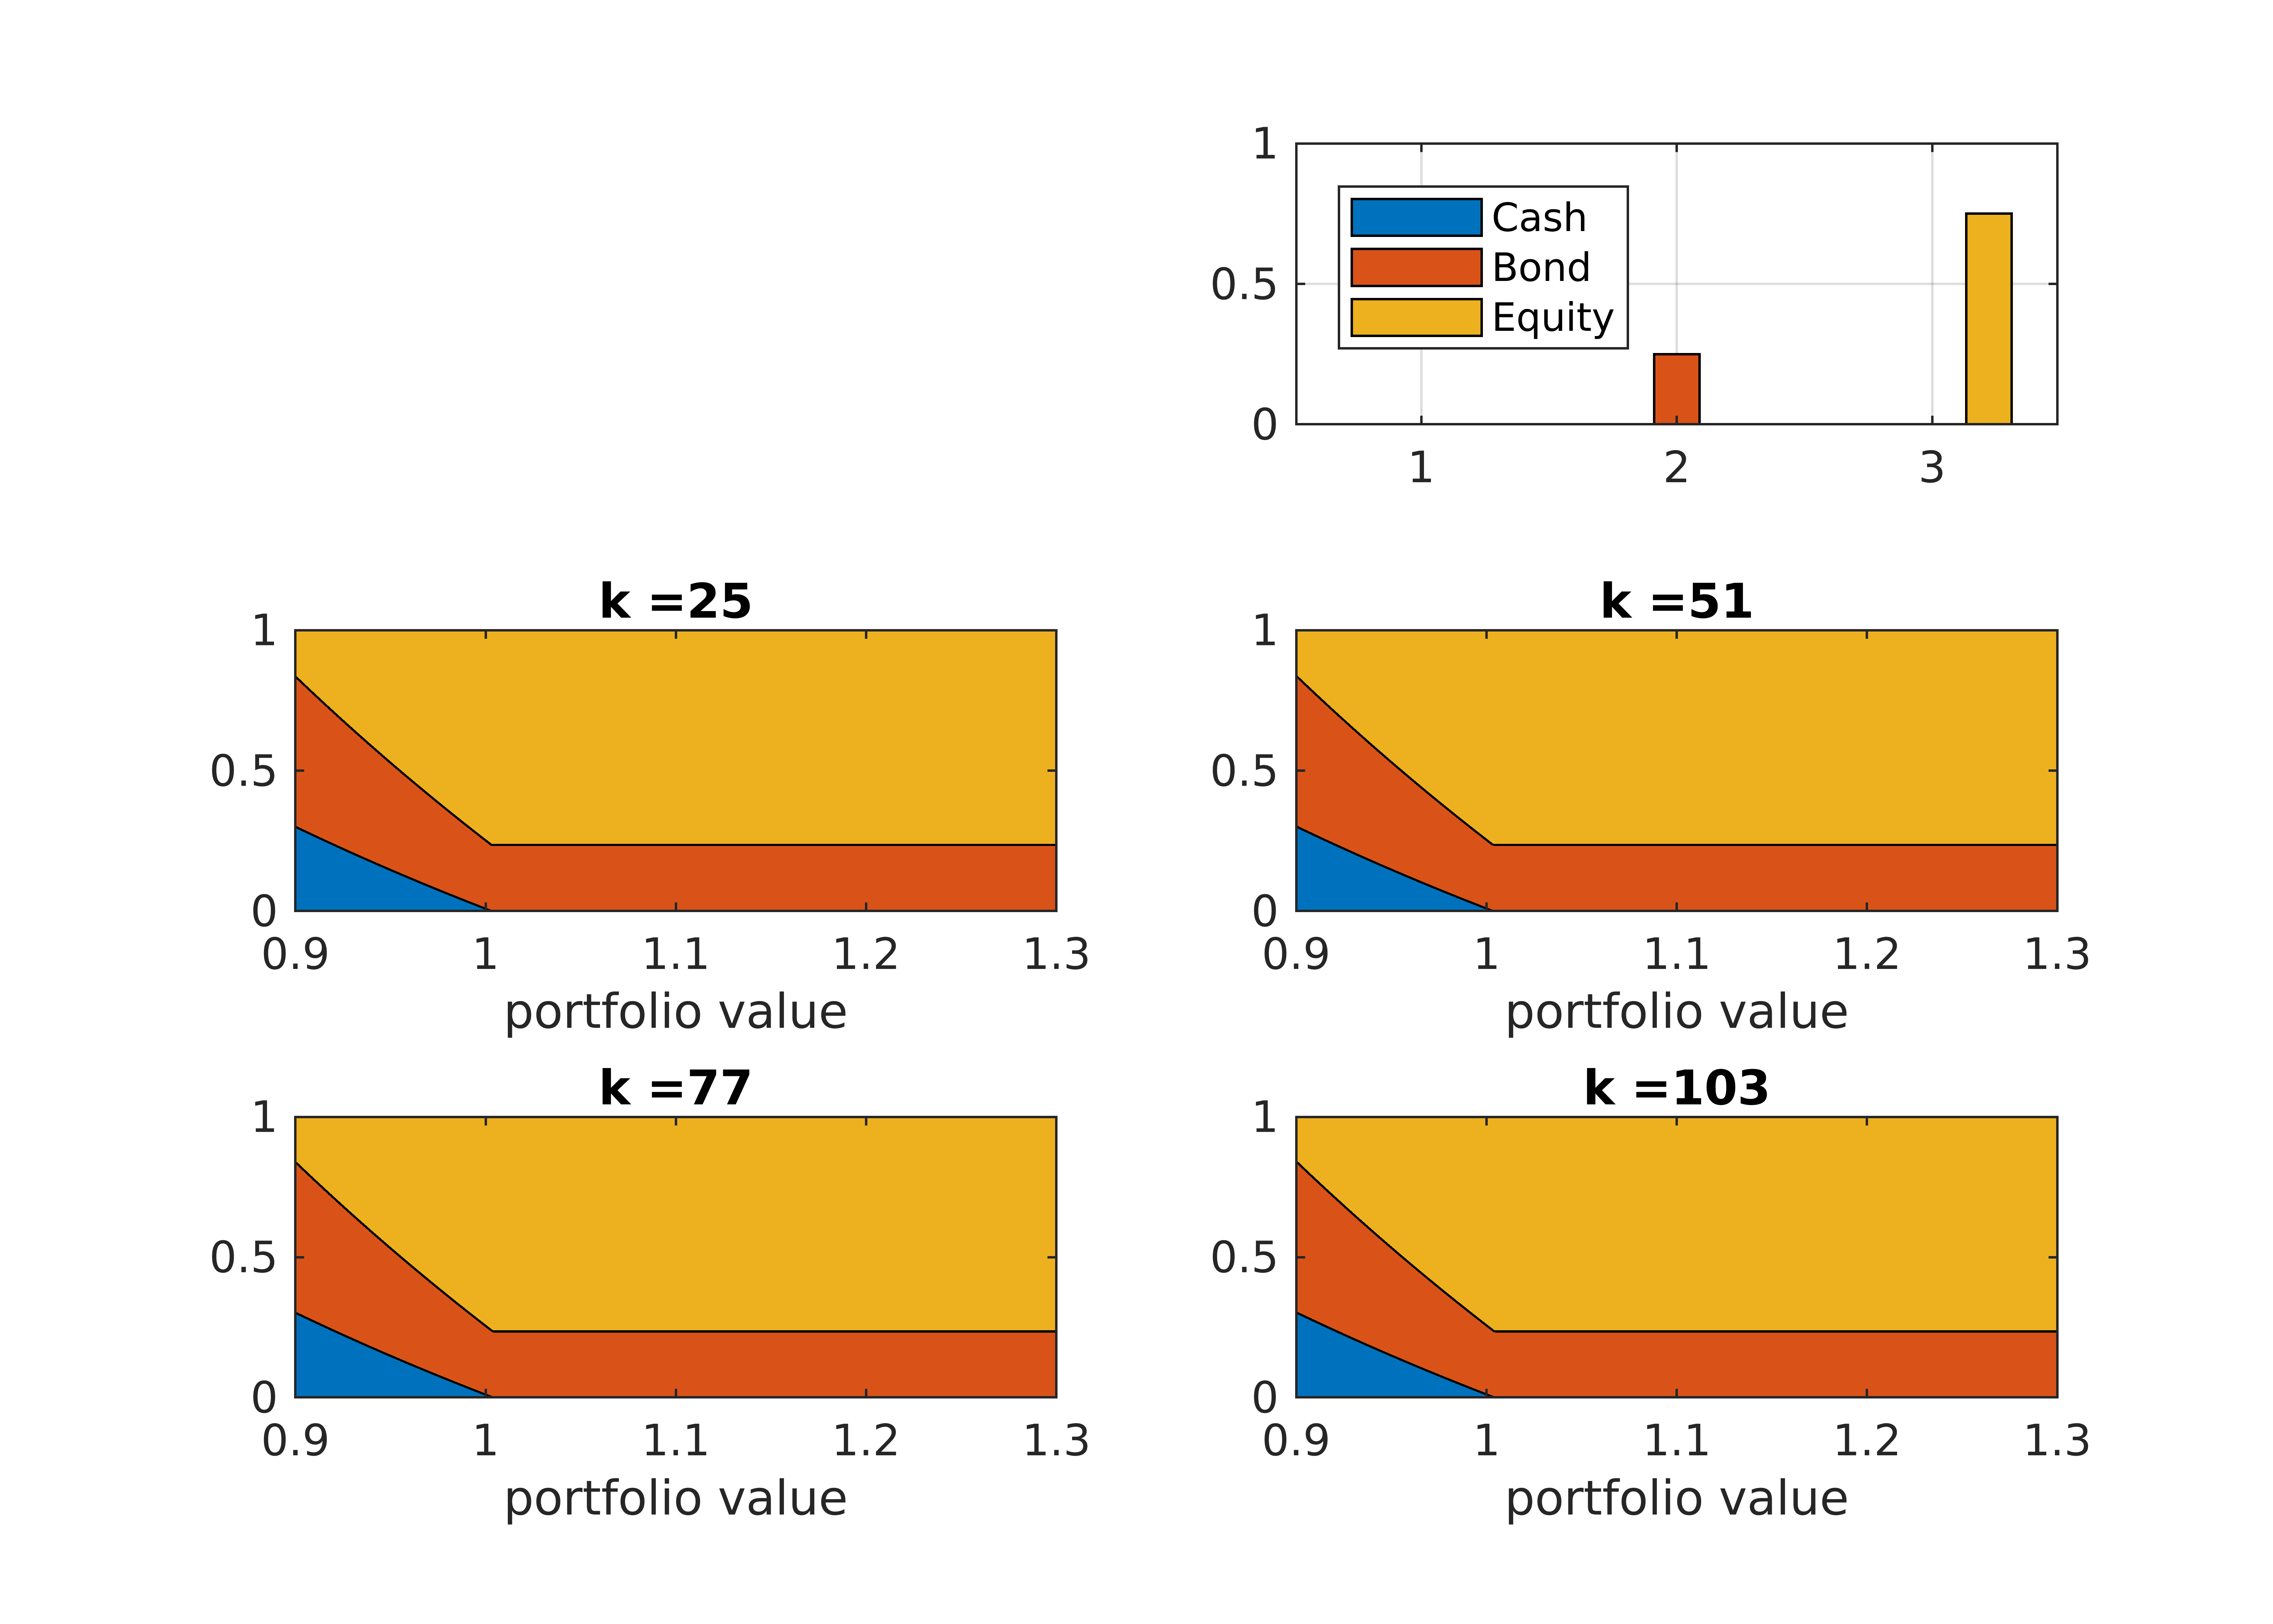
\includegraphics[scale = 0.8]{Images/mapsCPPIMixturewk.png}}
	\caption{Optimal CPPI allocation maps, weekly rebalancing, GM model. An example of a convex strategy.}
	\label{fig:mapsMixtureCPPI}
\end{figure}


\begin{table}[]
	\centering
	\begin{tabular}{@{}lccc@{}} \toprule
		Statistic & ODAA & CPPI & Constant-mix \\ \midrule
		$p_{MC}$ &  78.93\%    &  52.70\%    &  61.41\%    \\
		\addlinespace[0.5em]
		Mean Return (ann) & 5.82\%  & 7.55\% & 10.05\%\\
		\addlinespace[0.5em]
		Volatility (ann) & 5.00\%  & 7.93\% & 13.21\% \\
		\addlinespace[0.5em]
		Median (ann) &	7.20\% & 7.35\% & 9.41\% \\
		\addlinespace[0.5em]
		Skewnwss & 0.700 & -0.010 & 0.0146 \\
		\addlinespace[0.5em]
		Kurtosis & 6.700 & 3.052 & 3.012 \\
		\addlinespace[0.5em]
		Monthly $V@R_{0.95}$ & 5.49\% & 5.51\% & 9.42\%\\
		\addlinespace[0.5em]
		Max Drawdown & 43.39\% & 25.77\% & 45.80\% \\
		\addlinespace[0.5em]
		Mean Drawdown & 1.97\% & 2.12\% & 4.20\% \\
		\addlinespace[0.5em]
		Sharpe ratio & 1.163 & 0.951 & 0.760 \\ \bottomrule
		\addlinespace[0.5em]
	\end{tabular}
	\caption{Investment performance for strategies ODAA, CPPI and Constant-mix obtained via Monte-Carlo simulation ($\num{2e5}$ replications).}
	\label{tab:MC_statistics}
\end{table}



\begin{figure}[]
	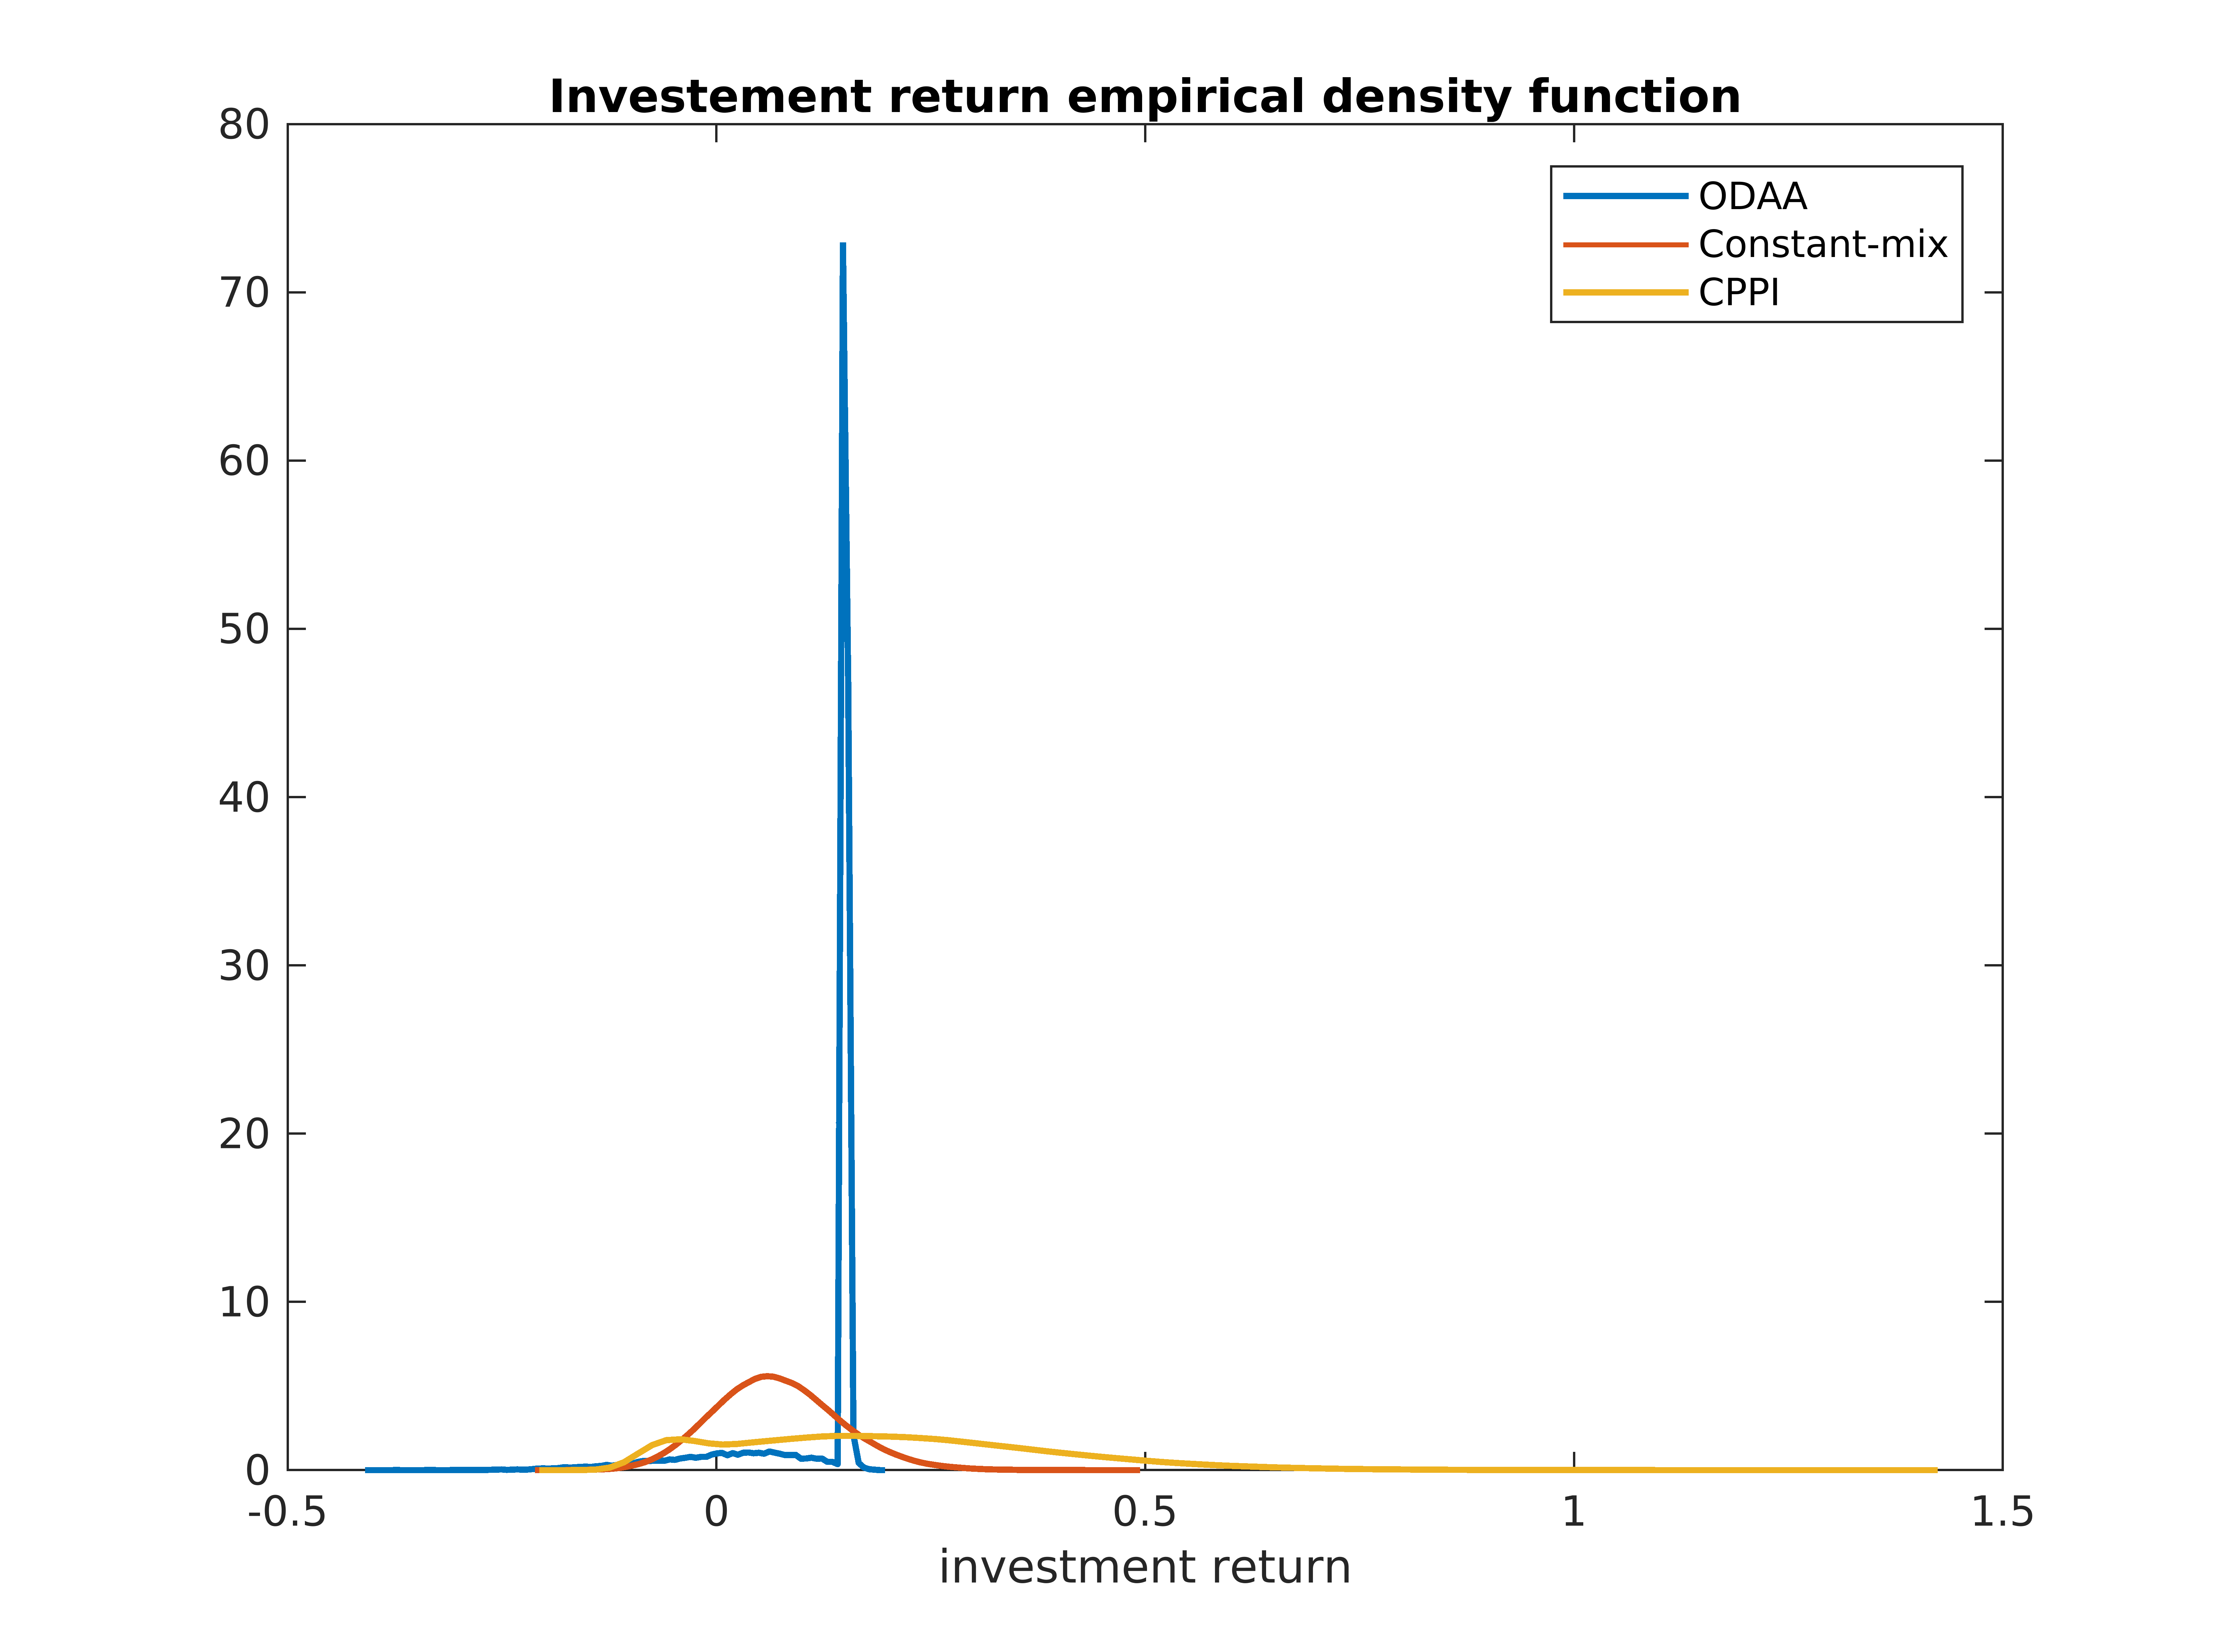
\includegraphics[scale = 0.6]{Images/DensitiesMixturewk}
	\caption{Empirical density functions of the 2-year return for the ODAA, CPPI and Constant-ix strategy.}
	\label{fig:epirical_densities}
\end{figure}